To satisfy the thesis objectives annunciated in the previous chapter, we combined application of four main knowledge areas: (i) the quality attributes, (ii) domain-specific design patterns, (iii) context-aware computing and (iv) component-based software engineering. The fundamental concepts of these knowledge areas are presented in the following sections, with respect to our objectives.

%\todo{Este capitulo esta flojo, le falta profundidad, debe quedar con al menos 10 paginas... debes tener cuidado con las citas bibliograficas. El bib tenia varios warnings, corregi varios, pero quedan algunos. Cuando adiciones, verifica al compilar los warnings. Los que estan, ya estan bien, excepto los dos warnings que quedaron.}

\section{Quality Attributes}
\label{subsec:qa}
Every software system implements a set of functionalities, which ideally correspond to the set of functional requirements requested by the stakeholders. However, this set of requirements is not the only software concern. Complementary, the constraints with which these functionalities must be performed and delivered constitute the list of non functional requirements that the software system should meet. Among these non functional requirements are the software quality attributes, for example, the maximum deadline of response to any request or the availability of the software services. Quality attributes are an important concern in the software engineering community because systems often have to be redesigned due to quality attributes deficiencies \cite{Bass:2003:SAP:773239}. For example, the web services have become to be a tool to perform transactions among clients and suppliers \cite{pertet2005causes}. If many client connect to the offered service of the supplier to buy his goods concurrently, then, his system could be overloaded if his current hardware and software architecture can not support a big amount of clients buying concurrently. Each second of the system is down could mean a high cost for the supplier (could be thousand of dollars) because he could lost not only sales and but also clients. To avoid this situation we could add the scalability quality attribute at system architecture but this imply a redesign that could be more expensive that the original system. The supplier would have not incur on an over cost if the scalability quality attribute had have been considered since beginning system construction.

In the before case, many quality attributes could be considered, such as, performance, availability, scalability, security, reliability, and capacity. The relevant quality attributes for a given system depend on its characteristics and constraints. Thus, to achieve an expected quality level of any quality attribute depends on how the system functions are implemented and designed. Achieving quality attributes also depend on software implementation, and its deployment. For example, performance depends on (i) communication among components, (ii) functionalities provided by each component, (iii) shared resources location, (iv) algorithms implementing functionalities, and (v) coding of these algorithms. In light of this, there are many aspects to consider when aiming at achieving a specific level of a quality attribute.

In this thesis we are focused on the impact that domain-specific design patterns have on performance factors with the aim of regulating the fulfillment of performance levels in particular self-adaptive systems.


\subsection{The Performance Quality Attribute}
\label{subsec:performance}
The performance quality attribute is defined as \textit{"The degree to which a system or component accomplishes its designated functions within given constraints, such as speed, accuracy, or memory usage."} \cite{barbacci1995quality}. This quality attribute is related to how much time it takes a system to execute functionalities in response to events. There are many kinds of events, such as interrupts, messages, requests from users, among others. The two main factors that make this quality attribute complex are; the amount of event sources and  event arrival patterns. For example, an event source is the user applications. The event arrival patterns may be characterized as periodical, sporadic or stochastic. Periodical events have a repetition pattern and possibly a deadline, whereas stochastic events occur according to a probabilistic distribution; sporadic events are those not categorized as neither periodical nor stochastic \cite{Bass:2003:SAP:773239}.

Because of its characteristics, performance has different aspects to quantify, through which it can be measure. These aspects are all known as sub-attributes or performance factors. The main performance sub-attributes are the following:

%\todo{A esto le falta detalle, por ejemplo, las unidades en que se mide, o como se mide}
%\renewcommand{\theenumi}{\thesubsection.\arabic{enumi}}
\begin{itemize}
	\item Throughput: The amount of events processed by unit time. The unit measure of this performance factor depends on the evaluated event, for example, the sorting algorithm could be measured as the sorted lines by milliseconds, the sorted files by seconds, or the sorting requests by minutes.  The way to measure this factor depends on the measure unit selected, for example, if the sorted files by seconds was selected, then, one way to perform the measurement is to ask to the system each second how many files have been processed. However, this measure could be not accurate because files that to start to be processed in a second would be attributed to other second where processing going to finish. For example, 5 files start to be processed in the first second but only 3 finish, in the next second finishing the other 2 files and to start 4 files and all to be whole processed. Throughput in the first second is 3 files/second, but in the next second is 6 files/second. Due to this situation before to measure the throughput factor an analysis of this factor behavior in the specific environment should be performed.
	\item Response Time: The elapsed time among an event arrival and the system response (also known as latency). Its unit measure is determined by the time used to process an event, that is, depend on the event kind. For example, to sorted a file could needed many minutes, so milliseconds should not be used. Another example is a system interrupt is executed in milliseconds, therefore, minutes should not be used to measure this performance factor. To measure the latency only one event should be sent to the system and it is important that the system is executing normally (i.e., processes that are not executed usually by the system, for example, a complicated programed task that only is executed one time on the day).
	\item Deadline: Constraint of time to complete an event processing. This factor should be defined and it should not be measured. For example, In windows operating system sometimes an event may not processed correctly so the operating system asking to the user after a time if it should finishing the event process or waiting that the event may be processed. To define this factor the latency factor could be used a reference time.
	\item Jitter of Response: Latency variation. The latency variation could show the system stability. If the system is not stable it could indicate that there are factors that are affecting the system performance. This performance sub-attribute is measured in the same measure unit that the latency sub-attribute. To measure this sub-attribute the latency sub-attribute is measured as a standard deviation of the latency so at least three data should be collected.
	\item Missing rate: Amount of missed events per unit time. To measure this performance sub-attribute is a complicated task due to the system does not know how many request are sent to it. A possible strategy to measure it is to implement a queue that allow to receive all request although not all could be processed. This sub-attribute have not an unit measure.
	\item Unprocessed rate: Amount of unprocessed events per unit time. This performance sub-attribute can be calculated as the events amount arrived minus the events amount processed. This sub-attribute have not an unit measure.
\end{itemize}
%\renewcommand{\theenumi}{\thesection.\arabic{enumi}}

\section {Domain-Specific Design Patterns}
Design patterns are typical solutions for recurrent and well-known engineering problems, in particular contexts. Design patterns usually are described in terms of (i) the problem, (ii) the applicable context, (iii) the intent, (iv) the forces, (v) the solution structure, and (vi) the solution behavior. However, these elements vary according to the pattern author. Design patterns should have been used thoroughly before being considered as such. Additionally, they should be applicable according to their intended context and problem. 

Despite of the elements used to describe a design pattern, it is not trivial to define whether they are better for an application area or another, they being considered as independent of domain of application \cite{gustavsson2002domain}. In light of this, the term domain-specific design pattern was introduced. Conceptually, this term groups design patterns that are, in some way, targeted for a particular domain. For example, real-time design patterns \cite{douglass2003real}, architecture design patterns \cite{kuchana2004software}, or Service Oriented Architecture (a.k.a. SOA) design patterns \cite{erl2008soa}. In this thesis the specific domain of interest for design patterns is performance. Therefore, we need a catalog of design patterns that address performance problems. These design patterns must have as objective to improve some of performance factors mention in section \ref{subsec:performance}, in this way, we can study how much the performance domain-specific design patterns could influence the performance factors. 

\section {Context-Aware Computing}
\label{subsec:contextaware}
Humans interact with their surrounding context in a natural way and under many circumstances and assumptions. Among these circumstances we count, for instance, the language, the understanding about world, implicit understanding of situations, and unconscious environment monitoring. However, computing systems have not the same \textit{``natural understanding''} about their context. According to Merriam-Webster context is defined as \textit{``the interrelated conditions in which something exists or occurs.''}, this is a wide definition. Villegas et al. \cite{villegas2013context} defines context as \textit{"Context is any information useful to characterize the state of individual entities and the relationships among them. An entity is any subject which can affect the behavior of the system and/or its interaction with the user. This context information must be modeled in such a way that it can be pre-processed after its acquisition from the environment, classified according to the corresponding domain, handled to be provisioned based on the system’s requirements, and maintained to support its dynamic evolution".} Thus context information includes, (i) computing environment (e.g., available CPUs, devices accessible for user input and display, network capacity, connectivity, and costs of computing), (ii) user environment (e.g., location, collection of nearby people, and social situation), and (iii) physical environment (e.g., lighting and noise level).

The context information is represented through context variables. A context variable represent a characteristic that is relevant to its context. For example, If our interest environment is the performance quality attribute some context variables could be the available processors, the available ram memory, or the available bandwidth. Each one of these characteristics could take their own values, using different measurement units and different ways to be measured, but all of them affect the performance quality attribute. Due to each one could influence in the performance in different measure so they should be studied as context variables. 

The context variables should be identified, defined, measured, and finally we could be studied the way that they interact and affect their environment. Each environment or study case could have their own relevant context variables, this is why the context variables should be identified. After to identify the context variables, these should be defined to avoid ambiguities, for example, the users amount context variable. This variable in a computing environment could represent the concurrent users for a web application but in a medical environment could represent the people attended by doctors in an any day. After to define the context variable, it needs to be measured depending on the definition of each variable (i.e., depend on its measurement unit and its way to be measured). If data about context variables is collected, it could be analyzed to discover the way that they interact and affect their environment.

Traditionally, we interact with computing systems through a keyboard and mouse, therefore, all information that these systems have about their surroundings are provided by these media. This is only one of causes whereby  the computing systems are not enabled to even monitor context. The context-aware computing not only is focused on how to make computing systems aware of context, but how to adapt to it.  Context-aware computing has become somewhat synonymous with other terms \cite{dey2016context}: adaptive, reactive, responsive, situated, context sensitive, and environment directed computing. Because of the amount of information context surrounds any application, context-aware computing is not a trivial knowledge area. Currently, there are many questions and challenges still to be solved.

The performance domain-specific design patterns specify the performance quality attribute as the most important context variable, because it defines where these should be applied. However, according to the context definition above mentioned there could context variables that can affect performance and they have been not identified on the context defined by design pattern.  As result of this, one challenge of this thesis is to study what is the quantitative relationship between the performance domain-specific design patterns and specific context variables.

%\todo{Hay que definir que es una variable de contexto, por que es importante, como se mide, ejemplos, etc.}


\section {Component-Based Software Engineering}
Doug Mcllroy introduced the software component concept in the first conference of software engineering (SE) in 1968 \cite{softwareComponents}. The concept of software components has turned into a principle of software engineering, as a generalization of modularity, and backed in the phrase "divide to conquer". This phrase makes reference to divide a problem into smaller problems to understand and solve it more easily. At some point, the solution of these smaller problems is manageable and can be represented by single components. In 1998, Component-Based Software Engineering (CBSE) was introduced as a sub area of SE. The CBSE paradigm has three main objectives: (i) to develop components as reusable entities, (ii) to develop software based in pre-existing components, and (iii) to evolve applications based in the replacement of components and their relationships \cite{softwareComponents}. 

CBSE has four principles to develop software: (i) re-usability, (ii) substitutability, (iii) extensibility, and (iv) composability. Each component has well defined responsibilities to accomplish these principles. To accomplish these principles, components are implemented as gray boxes with well defined services and exposed properties. These components can communicate with others through direct wires or indirect bindings with protocols such as SOAP, RMI, JMS, and REST.  Moreover, composability among components is hierarchical, that is, one component can contain and be implemented with other components. In this case, this component is called composite \cite{tamura:2012:QoS-CARE}.

The CBSE paradigm has been used widely in software engineering, including self-adaptive systems. The component approach allows to abstract the system goals at the component-level to support reconfiguration (i.e.,  create, replace, or delete components, wires, or bindings) at run-time. Thus, this abstraction provides the foundation for building self-adaptive systems.

%For this reason, this thesis is focused in specifically to produce knowledge that can be used to determine what changes through component-based reconfiguration at runtime could be useful to maintain the expected levels of quality attributes.

\subsection {The FraSCAti SCA Component Implementation}
\frascati{} is an implementation of the  Service Component Architecture (SCA) specification \cite{seinturier2012component}. SCA is a set of specifications based on Service-Oriented Architecture (SOA) and Component-Based Software Engineering (CBSE) principles, used to build software applications with distributed components. 

\frascati{} is a open source and multi-scale middleware to develop and execute distributed SCA applications. Additionally, it offers capabilities such as introspection and primitive components reconfiguration at runtime (i.e., create, remove, or modify components, wires and bindings). Through these capabilities dynamic reconfiguration is possible. The dynamic reconfiguration is needed to adapt systems to their context without to stop the systems operation.  In other words, these capabilities are required for leveraging context knowledge in order to reconfigure SCA systems. 

In \frascati{} each component is wrapped in a \frascati{} container that give to the component 7 services needed to offer the capabilities above mentioned \cite{seinturier2009reconfigurable}. 

\begin{itemize}
	\item Component Wiring: This service allows to the components query, register and remove wires although a SCA application is running.
	
	\item Component Instantiation: This service allows to instantiate each component according to only one of the modes proposed by SCA specifications (i.e., Stateless, request, conversation, and composite).
	
	\item Component Property: This service allows setting and getting values established as component properties, for example, the component name or the component host.  
	
	\item Component Identity: This service allows querying the set of provided services and required references of each component, additionally, this manages the components identity. That is, it allows discover dynamically requirements (i.e., references) and capabilities (i.e., services) of components.
	
	\item Component Hierarchy Management: This service allows to manage the hierarchical model proposed by the SCA specifications. That is, components can be composed by other components, these are called composites. So, there are primitive components and composites. This service give the component two main functionalities, (i) adding / querying / removing the subcomponents of a composite, and (ii) retrieving the parent of any component. 
	
	\item Component Lifecycle: This service allows to ensure that reconfiguration capabilities are executed in a safe way avoiding errors and inconsistencies through the component lifecycle control. That is, although reconfiguration operations usually are executed in multithread environments, this service delimits strictly the time intervals where a reconfiguration operation can be executed without affect the user requests.   
	
	\item Intent Management: This service allows to manage the non-functional properties of a SCA component through annotations mechanism, for example, @Requires annotation to manage the required references.
	
\end{itemize}


\subsection {The ICE Component Implementation}

Ice is an RPC framework with support for many languages (e.g., C++, C\#, Java, JavaScript, and Python) and operating systems (e.g., windows, linux, and Mac OS). Ice uses remote procedure calls (RPC) to realize communication between distributed components. 

Ice defines its own Interface Definition Language (IDL), Slice. This is intuitive and provides a rich set of data types that can be mapped to all supported languages. Additionaly, Ice allows synchronous and asynchronous invocations using TCP, UDP, SSL/TLS, and WebSockets. Ice was designed for applications with requirements on performance and scalability, using an efficient binary protocol to minimize CPU, memory, and bandwidth consumption.

\section {Autonomic Computing and Self-Adaptive Software Systems}

Autonomic computing and self-adaptive software systems are the inspiration and fundamental areas required to solve the stated problem of this thesis. We describe their related main concepts in the following.

\subsection {Autonomic Computing}
The vision of autonomic computing was proposed by Kephart and Chess in 2003 as mentioned previously in the section \ref{sec:motivation}. This vision is an anticipated answer to the problem of continuous systems growth, both in complexity and quantity. The main problem of this growth is that in some years there will be not enough system administrators to maintain systems in operation in the world. Consequently, the autonomic computing goal is that systems are enabled to perform the basic administrative functions themselves, autonomously. Autonomic computing is inspired in the autonomic nervous system that governs the basic human body functionalities such as breathing, maintaining heart rate and body temperature, among others. These functionalities do not need the attention of the brain's conscious functions exactly as the envisioned autonomic computing systems should not need system administrators to perform basic system functionalities of management.

In summary, the main principle of autonomic computing is self-management. Self-management implies that systems should maintain and adjust their operation when facing changes in components, workload demands, and external conditions that produce failures in the system's software or hardware. In order to perform functions such as creation, modification or deletion of components autonomously, systems should be equipped with capabilities such as self-configuration, self-adaptation, self-healing, self-optimization, self-protection, and other autonomic functions \cite{autonomiccomputing}.

The architecture proposed for implementing self-managed systems is based on the feedback loop model of control theory, and its adaptation for computing systems, the MAPE-K loop \cite{villegas-et-al:2017-architecting-SwSystems-for-self-adaptation}\cite{SEFSAS3:2017:challenges-assurances}\cite{SEFSAS3:2017:what-can-control}. As illustrated in Figure \ref{fig:mape-k}, the MAPE-K loop is composed of five elements: (i) monitor, (ii) analyzer, (iii) planner, (iv) executor, and (v) knowledge base.\\

%\todo{Esta descripcion hay que ponerla en bullets, por separado, y con mas detalle. Luego, explicar que la intencion es concentrarse en el K, con el fin de establecer una base inicial de K que sirva para futuros sistemas basados en MAPE-K donde el performance es un concern importante.}

Each element has a specific function in the loop.
\begin{itemize}
	\item The knowledge base: It supports the other elements' functionalities with the required information for each one. This element is transversal to all other MAPE-K loop elements due to this can have relevant information for each element. For example, how the monitor element could measure a context variable or which could be the best strategy to the executor element deploy a planner's plan.
	\item The monitor: It collects information about internal and external relevant context. To collect the relevant information monitors should be designed, each one depends on the context variable to measure (This information could be queried from the knowledge base element). This information represents the control symptoms (i.e., current system state), which will be compared with the reference control input (i.e., wanted system state).
	\item  The analyzer: It computes a control error signal and determines whether an adaptation is required. Additionally, it has the required information to identify which could be the problem cause, thanks to the monitor information and the knowledge base element.
	\item  The planner: It synthesizes control actions will be executed in the target system (i.e., the system under control) based on the information provided by the analyzer. These actions could be queried to the knowledge base element. 
	\item The executor: It executes the actions determined by the planner element, it tries to execute these actions without affecting the system users during it process. This element could query to the knowledge base element about how carry out the required actions in the best way.
\end{itemize}

Our intention in this thesis is focused on gathering information for The Knowledge Base Element with the aim of establishing an initial base for this element. This initial base could support future systems based on the MAPE-K loop where the performance would be an important concern.

\begin{figure}[ht!]
	\centering
	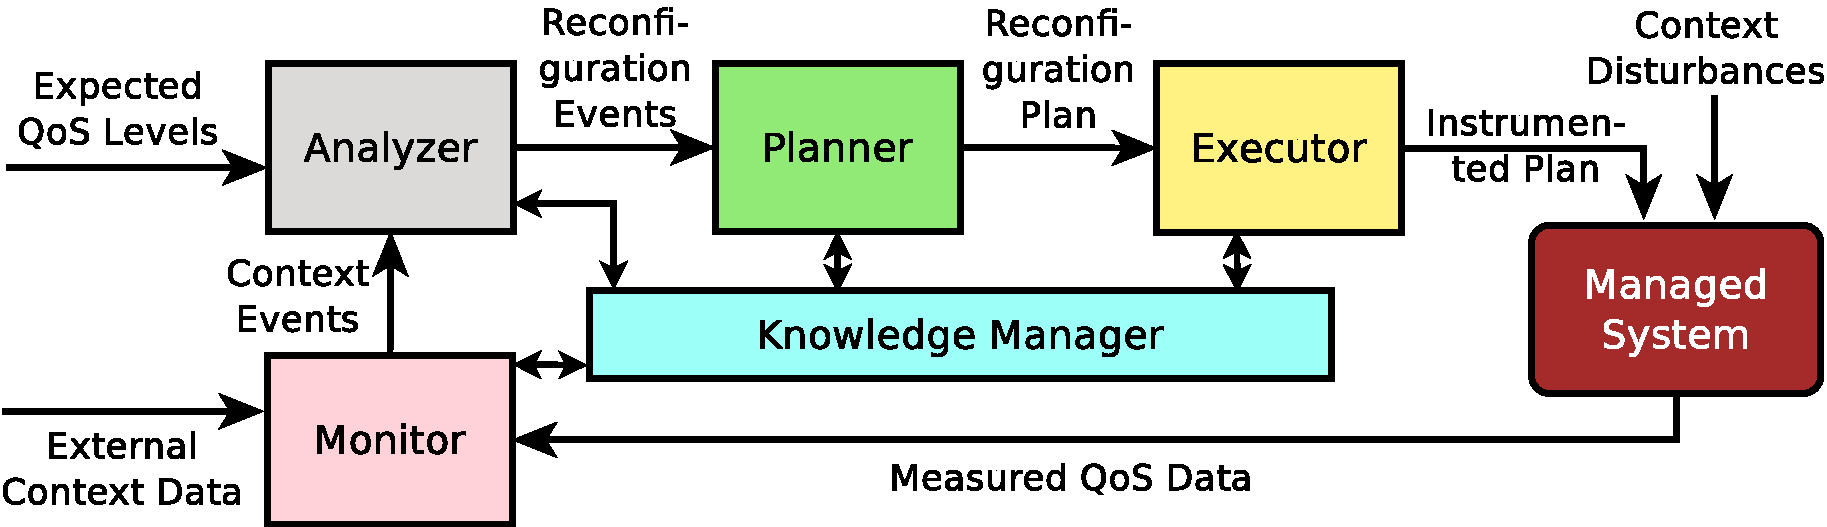
\includegraphics[width=0.95\textwidth]{fig/fback-loop-delta-dist}
	\caption{The MAPE-K reference model \cite{tamura:2012:QoS-CARE}}
	\label{fig:mape-k}
\end{figure}

\subsection {Self-Adaptive Software Systems}
As aforementioned in this document, self-adaptation is a capability of self-managed systems. Self-adaptive software systems are able to evaluate their own behavior and modify it in response to changes in their context (i.e., when these changes may imply that the system goals could not accomplished) or when achieving a better performance is possible \cite{tamura-et-al:2014:QoS-Contract-Preservation}\cite{villegas-et-al:2011:on-designing}. Because of this, self adaptive software systems are equipped with self monitoring components, analyzers, planners and executors. That is, they are usually based on the MAPE-K loop and technologies relying on component based architectures. Self-adaptive systems have been studied and applied in a wide variety of areas, such as systems evolution, object-oriented programming, autonomic computing, among others \cite{SEFSAS3:2017:what-can-control}\cite{villegas-et-al:2017-architecting-SwSystems-for-self-adaptation}\cite{Munoz-et-al:2015:refas-splc}\cite{Munoz-et-al:2015:variamos-splc}. However, the self-adaptive term is hard to distinguish from other terms, such as autonomic computing and self-management. According to \cite{Salehie:2009:SSL:1516533.1516538} the main difference between these terms is that autonomic computing includes a hierarchical set of layers required to administrate a software-intensive system: (i) application(s), (ii) middleware, (iii) network, and (iv) operating system, whereas self-adaptive systems are more limited and they only include layers (i) and (ii). However, in many cases these terms are used interchangeably.\\

Despite of there are numerous research about the Self-Adaptive software systems still there are many challenges around this topic \cite{de2013software}. The main challenges identified are:

\begin{itemize}
	\item Modeling dimensions: The objective of this challenge is to design models where a wide amount of systems properties could be represented to support the analysis and decision making processes.
	\item Requirements: The objective of this challenge is to capture the uncertain of any system through a language in an abstract level and interpreting this uncertain as a requirements collecting phase.
	\item Engineering: The objective of this challenge is to explicit the control loop role through the life-cycle of self-adaptive software systems (i.e., requirements, analyses, design, development, deployment, and operation of not only the system but also the control loop).
	\item Assurances: The objective of this challenge is to develop models that allow supplement the traditional V\&V methods to respond effectively to the dynamic context of the self-adaptive software systems.
	\item Design space for adaptive solutions: The objective of this challenge is to define a design space during the life-cycle of the self-adaptive software systems and the decisions that the software architect should address. In traditional life-cycle this space and these decisions are distributed through all process but these are centered in the analysis and design phases. However, in the self-adaptive software systems is more complicated to define this space due to its dynamic character.
	\item Processes: The objective of this challenge is to propose a process to develop a self-adaptive software system, this process should considerer dynamism involved by self-adaptive software systems.
	\item From centralized to decentralized control: The objective of this challenge is to design control schemes for centralized and decentralized structures defined a systematic way for software adaptation.
	\item Practical run-time verification and validation: The objective of this challenge is to investigate V\&V methods that allows gathering inferential assessment data to provide trust in self-adaptation process.
\end{itemize}

\subsection{Self-* Properties}

%\todo{DEBES reescribir los parrafos de esta seccion, porque son copy-paste de otro paper}

Self-* properties are the properties to be maintained by adaptation processes, introduced by Kephart and Chess in the vision of autonomic computing \cite{autonomiccomputing} in order to specify the aspects or attributes of self-managed systems, these are defined as follows: \\

\noindent\textbf{Self-Configuring.} This property defines that system must configure dynamically to accomplish with high-level policies specified in the service level agreements (SLAs). \\

\noindent\textbf{Self-Optimization.} This property defines that system must monitor and tune itself in an automatic way with the aim of improve its operation to satisfy needs of the end-user and business goals.\\

\noindent\textbf{Self-Healing.} This property defines that system must detect, diagnose, and repair any fail or malfunction of software found itself without the end-user perceives it or to affect the system execution. \\  

\noindent\textbf{Self-Protection.} 
This property defines that system must anticipate, detect, and identify potential threats that arise in its internal or external context and protect itself of them. \\

In terms of the self-* properties, our project will help in the advance of the achievement of the \textit{Self-Configuring} property, since the characterization of the system response in terms of latency and throughput performance factors of the relationship between design patterns and context-variables may guide the construction of the knowledge base component of SAS systems.


%\section {The \qoscare{} Framework}
%\qoscare{} is a reliable and robust reconfiguration framework that preserves QoS contracts in component-based software applications, which resulted from the PhD Thesis of Tamura \cite{tamura:2012:QoS-CARE}. The main goals of this thesis are: (i) to characterize properties of SAS systems and (ii) to provide a comprehensive solution to fulfill QoS contracts and preserve their fulfillment through dynamic reconfiguration. Relevant for our thesis proposal, the second specific result of Tamura's thesis is an evaluation framework for self-adaptive systems that defines a list of self-adaptation properties.

%In this section we focus on \qoscare{}, which is the implementation of a software architecture defined according to a formal model to preserve QoS contracts fulfillment. This  model is based in two formal systems: (i) the theory of Finite State Machines (FSM) and (ii) the Typed Attributed Graph (also called e-graph) Transformation System (TAGTS) theory. The theory of FSM is used to specify the semantics of QoS contracts, and modeling the fulfillment and unfulfillment states of QoS contracts. The TAGTS theory allows to model the reconfiguration operations using design patterns in reconfiguration rules due to TAGTS capabilities such as graph-based pattern-matching and transformation.

%\qoscare{} conceives the reconfiguration mechanism in an independent way of the managed software. Moreover, following the SCA standard, this mechanism is also independent of component runtime platforms. Therefore, we plan to use this framework to integrate the results of our proposal in it. \qoscare{} was designed to leverage domain-specific design-patterns at runtime, in general. Our aim in this thesis proposal is to parameterize and fine-tune its analyzer, planner, and knowledge-base with performance domain-specific design-patterns. 

%\section {Systematic Literature Reviews (SLR)}
%Systematic literature review is a methodology to perform rigorous reviews of the current state of studies about a particular topic developed in a particular area of knowledge \cite{keele2007guidelines}. The systematic literature review methodology defines a review protocol to assure the validity of a literature review because it must be repeatable by any researcher with the same results. This protocol is focused in defining a set of research questions that address the identification, evaluation, selection, and synthesis of relevant information.

%\section {PaSCAni}

%\section {Amelia}

\section{Chapter Summary}
This chapter summarizes all required concepts to approach this thesis. We start with the quality attributes (focused on the performance quality attribute and its sub-attributes), next, defining the domain-specific design patterns, after, we define the context-aware computing. These three concepts are the base of the problem defined in section \ref{sec:ProblemStatement} . Additional concepts required to understand the work carried out in this thesis are the component-based software engineering and the autonomic computing, specifically the self-adaptive software systems.